\documentclass[12pt, a4paper]{article}

% --- Packages ---
\usepackage[utf8]{inputenc}
\usepackage[T1]{fontenc}
\usepackage{geometry}
\usepackage{amsmath}
\usepackage{graphicx}
\usepackage{hyperref}
\usepackage{xcolor}
\usepackage{tikz}
\usetikzlibrary{positioning, shapes.geometric, arrows.meta, fit, backgrounds, calc}
\usepackage{booktabs}
\usepackage{array}
\usepackage{float}
\usepackage{listings}

% --- Colors ---
\definecolor{codegreen}{RGB}{0,128,0}
\definecolor{codegray}{RGB}{128,128,128}
\definecolor{codeblue}{RGB}{0,0,128}

% --- Code Listing Style ---
\lstset{
    basicstyle=\ttfamily\small,
    keywordstyle=\color{codeblue}\bfseries,
    commentstyle=\color{codegray}\itshape,
    stringstyle=\color{codegreen},
    showstringspaces=false,
    breaklines=true,
    frame=single,
    numbers=left,
    numberstyle=\tiny\color{codegray},
}

% --- Page Layout ---
\geometry{margin=1in}

% --- Document Metadata ---
\title{Beambot - Beamline Robotics Documentation}
\author{Aditya Bondada}
\date{\today}

\begin{document}

\maketitle

\section{Introduction}

\subsection{The Challenge: Sample Handling at Synchrotron Beamlines}

\subsection{Vision: Self-Driving Beamlines}

\subsection{The Gap: Integration Challenges}

\subsection{This Work: Beambot}

\subsection{Document Structure}

\section{Background}

\subsection{Synchrotron Beamlines}

\subsection{Robotic Manipulation}

\subsection{Existing Solutions}

\subsection{Technology Choices}

\section{System Architecture}

\subsection{High-Level Architecture}

\begin{figure}[H]
\centering
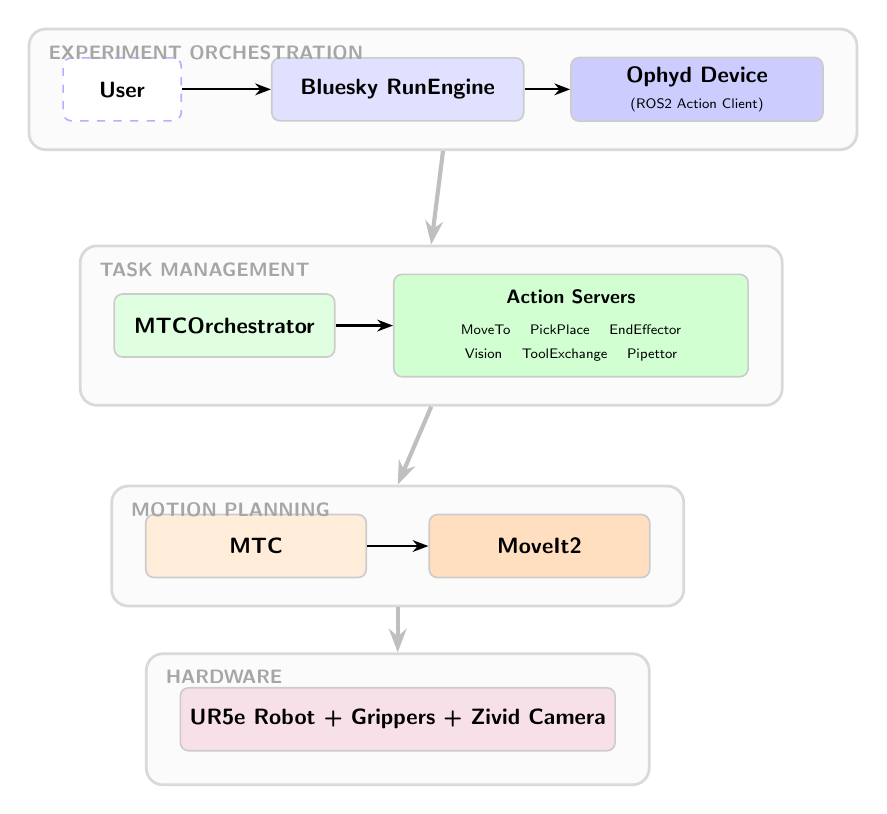
\begin{tikzpicture}[
    font=\sffamily\footnotesize,
    harrow/.style={-{Stealth[length=2mm]}, line width=0.8pt},
    varrow/.style={-{Stealth[length=3mm]}, line width=1.5pt, color=gray!50},
    box/.style={
        rectangle,
        rounded corners=3pt,
        minimum height=0.8cm,
        text centered,
        draw=gray!40,
        line width=0.6pt,
        fill=#1
    },
    groupbox/.style={
        rectangle,
        rounded corners=6pt,
        draw=gray!30,
        line width=1pt,
        inner xsep=12pt,
        inner ysep=10pt,
        fill=gray!3
    },
    grouplabel/.style={
        font=\scriptsize\bfseries\sffamily,
        text=gray!70
    },
    boxlabel/.style={
        font=\tiny\sffamily,
        text=gray!60
    }
]

% Define consistent width for all groups
\def\groupwidth{9cm}

% === GROUP 1: EXPERIMENT ORCHESTRATION ===
\node (user) [box=white, draw=blue!30, dashed, minimum width=1.5cm] at (-3.5,0) {\textbf{User}};
\node (bluesky) [box=blue!12, minimum width=3.2cm] at (0,0) {\textbf{Bluesky RunEngine}};
\node (ophyd) [box=blue!20, minimum width=3.2cm, align=center] at (3.8,0) {\textbf{Ophyd Device}\\\tiny(ROS2 Action Client)};

\begin{scope}[on background layer]
\node [groupbox, fit=(user)(bluesky)(ophyd), inner xsep=12pt] (group1) {};
\end{scope}
\node [grouplabel, anchor=north west] at ([xshift=4pt, yshift=-3pt]group1.north west) {EXPERIMENT ORCHESTRATION};

\draw [harrow] (user.east) -- (bluesky.west);
\draw [harrow] (bluesky.east) -- (ophyd.west);

% === GROUP 2: TASK MANAGEMENT ===
\node (orchestrator) [box=green!12, minimum width=2.8cm] at (-2.2,-3) {\textbf{MTCOrchestrator}};
\node (actions) [box=green!18, minimum width=4.5cm, minimum height=1.3cm] at (2.2,-3) {
    \begin{tabular}{c}
        \textbf{\scriptsize Action Servers} \\[2pt]
        \tiny MoveTo \quad PickPlace \quad EndEffector \\[-1pt]
        \tiny Vision \quad ToolExchange \quad Pipettor
    \end{tabular}
};

\begin{scope}[on background layer]
\node [groupbox, fit=(orchestrator)(actions), inner xsep=12pt] (group2) {};
\end{scope}
\node [grouplabel, anchor=north west] at ([xshift=4pt, yshift=-3pt]group2.north west) {TASK MANAGEMENT};

\draw [harrow] (orchestrator.east) -- (actions.west);

% === GROUP 3: MOTION PLANNING ===
\node (mtc) [box=orange!15, minimum width=2.8cm] at (-1.8,-5.8) {\textbf{MTC}};
\node (moveit) [box=orange!25, minimum width=2.8cm] at (1.8,-5.8) {\textbf{MoveIt2}};

\begin{scope}[on background layer]
\node [groupbox, fit=(mtc)(moveit), inner xsep=12pt] (group3) {};
\end{scope}
\node [grouplabel, anchor=north west] at ([xshift=4pt, yshift=-3pt]group3.north west) {MOTION PLANNING};

\draw [harrow] (mtc.east) -- (moveit.west);

% === GROUP 4: HARDWARE ===
\node (robot) [box=purple!12, minimum width=5.5cm] at (0,-8) {\textbf{UR5e Robot + Grippers + Zivid Camera}};

\begin{scope}[on background layer]
\node [groupbox, fit=(robot), inner xsep=12pt, inner ysep=12pt] (group4) {};
\end{scope}
\node [grouplabel, anchor=north west] at ([xshift=4pt, yshift=-3pt]group4.north west) {HARDWARE};

% === VERTICAL ARROWS BETWEEN GROUPS ===
\draw [varrow] (group1.south) -- (group2.north);
\draw [varrow] (group2.south) -- (group3.north);
\draw [varrow] (group3.south) -- (group4.north);

\end{tikzpicture}
\caption{Beambot software architecture: horizontal data flow within layers, vertical flow between architectural layers.}
\label{fig:software-stack}
\end{figure}

The system architecture is organized into four primary layers, each responsible for distinct functionalities within the overall system (see Figure~\ref{fig:software-stack}). The user / Beamline scientist interacts with the Bluesky RunEngine to define and execute experiments. 
This is the same interface used to control other beamline hardware, ensuring seamless integration into existing workflows. To facilitate this the ROS2 action client is wrapped as an Ophyd device - so it behaves like any other beamline hardware component.
The RunEngine sends high-level commands to the MTCOrchestrator, which manages task execution by coordinating various action servers. These action servers encapsulate specific functionalities such as moving the robot, picking and placing samples, vision processing, tool exchanges, and pipetting operations.
The MTC (Motion Task Compiler) layer translates high-level task commands into motion plans, leveraging the MoveIt2 framework for path planning and collision avoidance.
Finally, the hardware layer consists of the UR5e robotic arm, equipped with grippers and a Zivid 3D camera for visual feedback.

\subsection{Experiment Orchestration Layer}
The user / Beamline scientist interacts with the Bluesky RunEngine to define and execute experiments. The Ophyd device/ROS2 action client sends a JSON file that defines the experimentation task sequence  - e.g., load sample from position A, move to sample place position, change tool, etc. 
\subsection{Task Management Layer}

\subsection{Motion Planning Layer}

\subsection{Hardware Layer}

\end{document}
